\chapter{Imbangan Termodinamika dan Sistem Terbuka}\label{ch:b2:open-systems}

Termodinamika jilid Tahun 1 menggarap sistem tertutup ---
sejumlah massa gas yang tetap dalam sebuah silinder, yang dimampatkan, dipanaskan, dimuaikan. Tetapi
mesin yang sungguh memanaskan rumah kita, mendinginkan makanan kita dan membuat
listrik kita diseberangi sebuah \emph{aliran}: uap mengalir menembus
turbin sebuah pusat listrik dengan beratus kilogram tiap sekon, sebuah
zat pendingin beredar menembus kompresor, kondensor, katup dan
evaporator sebuah pompa kalor, udara mengalir menembus kompresor dan
ruang bakar sebuah mesin jet. Tiap komponennya adalah sebuah \emph{\omterm{def:b2:open-systems:cv}{sistem
terbuka}}, yaitu sebuah daerah ruang dengan materi yang masuk dan pergi, dan
hukum pertama dan keduanya harus ditulis ulang baginya. Penulisan ulangnya pendek
--- kuncinya adalah bahwa fluida yang didorong masuk ke sistemnya mengemban, di samping
energi dalamnya, kerja yang dilakukan untuk mendorongnya, itulah sebabnya
\emph{\omterm{thm:b2:open-systems:firstlaw}{entalpi}}, bukan energi dalam, merupakan energi alami sebuah aliran.
Bab ini menegakkan imbangan massa, energi dan entropi bagi
\omterm{def:b2:open-systems:cv}{sistem terbuka} dalam \omterm{def:b2:open-systems:cv}{aliran tunak}, menerapkannya pada piranti dasarnya ---
\omterm{prop:b2:open-systems:devices}{nosel}, \omterm{prop:b2:open-systems:devices}{katup cekik}, kompresor, turbin, \omterm{prop:b2:open-systems:devices}{penukar kalor} --- lalu merakit
piranti itu menjadi kedua daur yang diukur soal akhir pekannya: sebuah
pompa kalor dan sebuah pusat listrik tenaga uap.

\begin{omfigure}
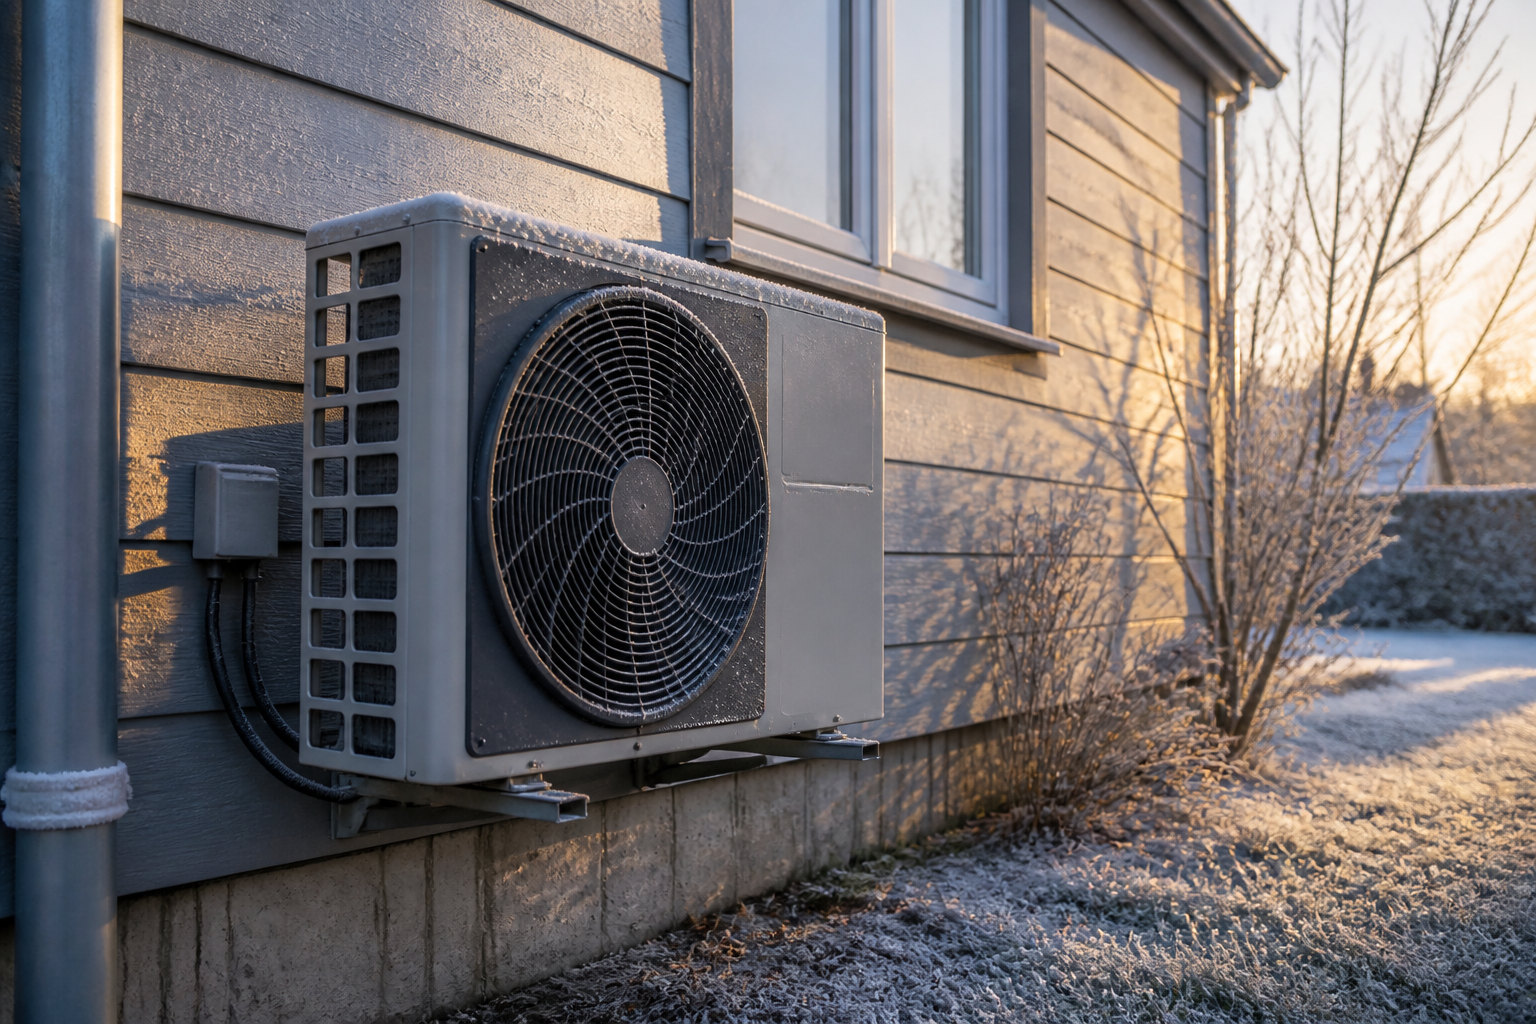
\includegraphics[width=0.58\linewidth]{images/book4/ai/b4-27-heat-pump-winter.png}

{\small Unit luar sebuah pompa kalor pada pagi musim dingin: sebuah kipas
menarik udara dingin melewati evaporatornya, dan di dalamnya sebuah kompresor, sebuah
kondensor dan sebuah katup memindahkan kalor itu, tiga atau empat kali lipat,
ke dalam rumahnya.}
\end{omfigure}

\section{Sistem terbuka dan imbangan massa}

\begin{definition}[Sistem terbuka, volume kendali, aliran tunak]\label{def:b2:open-systems:cv}
Sebuah \emph{sistem terbuka}\index{sistem terbuka} adalah sebuah daerah ruang yang tetap,
yaitu \emph{volume kendali}\index{volume kendali} $\Sigma$, yang dibatasi sebuah
permukaan yang menembusnya fluida masuk dan pergi (penampang masuk dan
keluar) dan yang menembusnya kalor dan kerja dapat dipertukarkan dengan
luarnya; kerja yang diterima lewat suku yang bergerak (sebuah poros, sebuah torak)
selain aliran itu sendiri adalah \emph{kerja berguna}\index{kerja berguna}
$W_{\text{u}}$ (kerja poros). Alirannya \emph{tunak}\index{aliran
tunak} bila setiap medan di dalam $\Sigma$ tak bergantung waktu: massa,
energi dan entropi yang termuat dalam $\Sigma$ lalu tetap.
\end{definition}

\begin{proposition}[Imbangan massa]\label{prop:b2:open-systems:mass}
Menembus sebuah penampang berluas $S$ yang fluidanya berkerapatan $\rho$ bergerak
dengan kelajuan rerata $c$ yang tegak lurus padanya mengalirlah \emph{debit
massa}\index{debit massa} $\dot m = \rho c S$ (dalam \unit{kg/s}). Dalam sebuah
\omterm{def:b2:open-systems:cv}{aliran tunak}, yang masuk itulah yang pergi: $\sum_{\text{msk}}\dot m = \sum_{\text{kel}}
\dot m$; bagi sebuah arus tunggal, $\dot m$ sama di masukan dan keluarannya,
$\rho_1c_1S_1 = \rho_2c_2S_2$ --- yaitu \omterm{thm:b2:fluid-kinematics:continuity}{persamaan kontinuitas}
\cref{ch:b2:fluid-kinematics} yang diintegralkan pada penampangnya.
\end{proposition}

\begin{proof}
Massa dalam $\Sigma$ tetap, jadi fluksnya saling mengimbangi.
\end{proof}

\section{Hukum pertama bagi sebuah sistem terbuka}

\begin{theorem}[Imbangan energi sebuah aliran arus tunggal yang tunak]\label{thm:b2:open-systems:firstlaw}
Bagi sebuah \omterm{def:b2:open-systems:cv}{aliran tunak} berdebit massa $\dot m$ yang masuk pada keadaan 1
dan pergi pada keadaan 2, sambil menerima daya berguna (poros)
$P_{\text{u}}$ dan daya termal $P_{\text{th}}$,
\[
\dot m\,\Big[(h_2 - h_1) + \tfrac12(c_2^2 - c_1^2) + g(z_2 - z_1)\Big]
= P_{\text{u}} + P_{\text{th}} ,
\]
atau, tiap satuan massa fluida yang menyeberangi sistemnya,
\[
\Delta h + \Delta\big(\tfrac12c^2\big) + g\,\Delta z = w_{\text{u}} + q .
\]
\emph{Entalpi}\index{entalpi (dalam sebuah aliran)} $h = u + Pv$ menggantikan
energi dalamnya: $Pv$ adalah \emph{kerja aliran}, yaitu kerja yang dilakukan
fluida hulunya untuk mendorong satu satuan massa masuk, dikurangi yang dilakukan untuk mendorongnya
keluar.
\end{theorem}

\begin{proof}
Ikutilah sistem tertutup yang terbuat dari fluida di dalam $\Sigma$ pada $t$ ditambah
bongkah $\dd m = \dot m\,\dd t$ yang hendak masuk; pada $t + \dd t$ ia
terdiri atas fluida di dalam $\Sigma$ (keadaan yang sama, \omterm{def:b2:open-systems:cv}{tunak}) ditambah
bongkah $\dd m$ yang telah pergi. Energinya berubah sebesar
$\dd m\,[(u_2 + \tfrac12c_2^2 + gz_2) - (u_1 + \tfrac12c_1^2 + gz_1)]$. Ia
menerima $P_{\text{u}}\dd t + P_{\text{th}}\dd t$, ditambah kerja gaya
tekanan di masukannya, $P_1S_1 \times c_1\dd t = P_1v_1\,\dd m$
(yang mendorong bongkahnya masuk), dikurangi yang di keluarannya, $P_2v_2\,\dd m$. Hukum
pertama bagi sistem tertutup ini, dengan $u + Pv = h$, memberi hasilnya.
\end{proof}

\begin{omfigure}
\begin{tikzpicture}[scale=0.95, >=stealth]
  \draw[thick, rounded corners=6pt, fill=omDef!8] (1.2,0) rectangle (6.2,2.6);
  \node[font=\scriptsize] at (3.7,1.9) {volume kendali $\Sigma$ (tunak)};
  % inlet pipe
  \draw[thick] (-0.6,0.5) -- (1.2,0.5); \draw[thick] (-0.6,1.1) -- (1.2,1.1);
  \fill[omExo!40] (-0.5,0.52) rectangle (0.1,1.08);
  \node[font=\scriptsize, above] at (-0.2,1.12) {$\dd m$};
  \draw[->, omExo, thick] (-1.4,0.8) -- (-0.6,0.8);
  \node[font=\scriptsize, left] at (-1.4,0.8) {$\dot m$, $h_1$, $c_1$, $z_1$};
  % outlet pipe
  \draw[thick] (6.2,1.5) -- (8.0,1.5); \draw[thick] (6.2,2.1) -- (8.0,2.1);
  \fill[omExo!40] (7.3,1.52) rectangle (7.9,2.08);
  \node[font=\scriptsize, above] at (7.6,2.12) {$\dd m$};
  \draw[->, omExo, thick] (8.0,1.8) -- (8.8,1.8);
  \node[font=\scriptsize, right] at (8.8,1.8) {$h_2$, $c_2$, $z_2$};
  % shaft
  \draw[->, omThm, very thick] (3.7,-0.8) -- (3.7,0) node[pos=0, below, font=\scriptsize] {$P_{\text{u}}$ (shaft)};
  \draw[->, omThm, very thick] (5.5,3.4) -- (5.5,2.6) node[pos=0, above, font=\scriptsize] {$P_{\text{th}}$};
  % pressure pushes
  \node[font=\scriptsize, omExo] at (0.3,0.2) {$P_1v_1$ mendorong masuk};
  \node[font=\scriptsize, omExo] at (7.2,1.2) {$P_2v_2$ mendorong keluar};
\end{tikzpicture}

{\small \omterm{def:b2:open-systems:cv}{Sistem terbuka} yang \omterm{def:b2:open-systems:cv}{tunak}: sistem tertutup yang diikuti selama $\dd
t$ adalah isi $\Sigma$ ditambah bongkah yang masuk, lalu isinya
ditambah bongkah yang pergi; kerja tekanan pada kedua penampangnya mengubah $u$
menjadi $h = u + Pv$.}
\end{omfigure}

\begin{remark}[Memakai hukum pertamanya]\label{rem:b2:open-systems:using}
Bagi sebuah gas ideal $\Delta h = c_p\Delta T$; bagi sebuah cairan $\Delta h \approx
c\,\Delta T + v\,\Delta P$ (suku keduanya adalah kerja pompanya); bagi sebuah uap
orang membaca $h$ dari tabel atau bagan. Suku kinetiknya biasanya
dapat diabaikan: pada \qty{10}{m/s}, $c^2/2 = \qty{50}{J/kg}$, melawan
\qty{1}{kJ/kg} bagi satu kelvin udara --- ia hanya berarti dalam \omterm{prop:b2:open-systems:devices}{nosel} dan
sudu turbin, yang kelajuannya mencapai beratus meter tiap sekon. Suku
potensialnya, $g\Delta z \approx \qty{10}{J/kg}$ tiap meter, berarti bagi
air dalam sebuah bendungan, tak pernah dalam sebuah daur gas. Dengan beberapa masukan dan keluaran
imbangannya berbunyi $\sum_{\text{kel}}\dot m\,h - \sum_{\text{msk}}\dot m\,h =
P_{\text{u}} + P_{\text{th}}$ (suku kinetik dan potensialnya diabaikan).
\end{remark}

\section{Hukum kedua bagi sebuah sistem terbuka}

\begin{theorem}[Imbangan entropi sebuah aliran tunak]\label{thm:b2:open-systems:secondlaw}
Bagi sebuah aliran arus tunggal yang \omterm{def:b2:open-systems:cv}{tunak} yang mempertukarkan daya termal
$P_{\text{th},i}$ dengan sumber bersuhu $T_i$,
\[
\dot m\,(s_2 - s_1) = \sum_i\frac{P_{\text{th},i}}{T_i} + \dot S_{\text{c}},
\qquad \dot S_{\text{c}} \ge 0 ;
\]
tiap satuan massa, $\Delta s = s_{\text{tukar}} + s_{\text{c}}$. Sebuah aliran
adiabatik yang terbalikkan bersifat \emph{isentropik}; sebuah aliran adiabatik yang sungguhan mempunyai $s_2 >
s_1$. \emph{Efisiensi isentropik}\index{efisiensi isentropik} sebuah
turbin adalah $\eta_{\text{T}} = w_{\text{nyata}}/w_{\text{s}} = (h_1 - h_2)/(h_1
- h_{2s})$ dan efisiensi sebuah kompresor $\eta_{\text{C}} = (h_{2s} - h_1)/(h_2 -
h_1)$, dengan $2s$ yaitu keadaan yang dicapai secara isentropik pada tekanan
keluaran yang sama; keduanya lazimnya $0.8$--$0.9$. Kerja yang hilang karena
ketakterbalikan, yang diacukan ke suhu lingkungan $T_0$, adalah
$T_0\,s_{\text{c}}$ tiap satuan massa.
\end{theorem}

\begin{proof}
Sistem tertutup yang sama seperti sebelumnya: entropinya berubah sebesar $\dd m\,(s_2 -
s_1)$, menerima $\sum P_{\text{th},i}\dd t/T_i$ dari sumbernya, dan
sisanya diciptakan.
\end{proof}

\section{Piranti dasar}

\begin{proposition}[Nosel, katup cekik, kompresor, turbin, penukar]\label{prop:b2:open-systems:devices}
Semuanya adiabatik kecuali dinyatakan lain, \omterm{def:b2:open-systems:cv}{tunak}, dengan suku kinetik dan potensial
diabaikan kecuali jika itulah pokoknya.
\begin{itemize}
\item \emph{Nosel}\index{nosel} (tanpa poros, tanpa kalor): $\tfrac12c_2^2 -
      \tfrac12c_1^2 = h_1 - h_2$ --- \omterm{thm:b2:open-systems:firstlaw}{entalpi} menjadi kelajuan; sebuah
      \emph{difusor} melakukan kebalikannya.
\item \emph{Katup cekik}\index{katup cekik} (katup, sumbat berpori; tanpa poros,
      tanpa kalor, kelajuannya kecil): $h_2 = h_1$, \emph{isentalpik}. Bagi sebuah
      gas ideal $T_2 = T_1$; bagi gas yang sungguhan suhunya umumnya
      turun (efek Joule--Thomson); bagi sebuah cairan dekat kejenuhannya
      sebagian menguap kilat menjadi uap --- yaitu katup pemuai setiap
      lemari pendingin.
\item \emph{Kompresor, pompa, turbin}\index{turbin} (mesin
      adiabatik): $w_{\text{u}} = h_2 - h_1$ --- positif bagi sebuah kompresor,
      negatif bagi sebuah turbin; bagi sebuah pompa cairan $w_{\text{u}} \approx
      v(P_2 - P_1)$, yang mungil karena $v$ kecil.
\item \emph{Penukar kalor}\index{penukar kalor} (dua arus, tanpa
      poros, adiabatik sebagai keseluruhan): $\dot m_{\text{a}}(h_{\text{a},2} -
      h_{\text{a},1}) = -\dot m_{\text{b}}(h_{\text{b},2} - h_{\text{b},1})$
      --- yang hilang dari yang satu diperoleh yang lain; pertukarannya menciptakan entropi
      kecuali arusnya bersuhu sama di mana-mana
      (aliran lawan menguranginya).
\item \emph{Ruang pencampur}: $\sum\dot m_{\text{msk}}h_{\text{msk}} = \dot
      m_{\text{kel}}h_{\text{kel}}$.
\end{itemize}
\end{proposition}

\begin{proof}
Masing-masingnya adalah hukum pertama dengan suku yang tak berlaku disetel nol.
\end{proof}

\begin{omfigure}
\begin{tikzpicture}[scale=0.85, >=stealth]
  % nozzle
  \draw[thick] (0,0.2) -- (1.6,0.55) -- (1.6,0.85) -- (0,1.2);
  \draw[->, omExo, thick] (-0.6,0.7) -- (-0.1,0.7);
  \draw[->, omExo, very thick] (1.7,0.7) -- (2.9,0.7);
  \node[font=\scriptsize] at (1.0,-0.35) {nosel: $h \to c^2/2$};
  % throttle
  \begin{scope}[xshift=4.6cm]
    \draw[thick] (0,0.4) -- (1.0,0.4) -- (1.0,0.55) -- (1.2,0.55) -- (1.2,0.4) -- (2.4,0.4);
    \draw[thick] (0,1.0) -- (1.0,1.0) -- (1.0,0.85) -- (1.2,0.85) -- (1.2,1.0) -- (2.4,1.0);
    \draw[->, omExo, thick] (-0.6,0.7) -- (-0.1,0.7);
    \draw[->, omExo, thick] (2.5,0.7) -- (3.1,0.7);
    \node[font=\scriptsize] at (1.2,-0.35) {katup cekik: $h_2 = h_1$};
    \node[font=\scriptsize] at (0.4,1.3) {$P_1$}; \node[font=\scriptsize] at (2.0,1.3) {$P_2 < P_1$};
  \end{scope}
  % turbine
  \begin{scope}[xshift=9.6cm]
    \draw[thick] (0,1.3) -- (0,0.1) -- (2.0,-0.3) -- (2.0,1.7) -- cycle;
    \draw[->, omExo, thick] (-0.7,1.0) -- (-0.1,1.0);
    \draw[->, omExo, thick] (2.1,0.3) -- (2.8,0.3);
    \draw[->, omThm, very thick] (1.0,-0.4) -- (1.0,-1.0) node[below, font=\scriptsize] {$w_{\text{u}} = h_2 - h_1 < 0$};
    \node[font=\scriptsize] at (1.0,2.0) {turbin};
  \end{scope}
  % exchanger
  \begin{scope}[yshift=-3.2cm]
    \draw[thick, rounded corners=4pt] (0,0) rectangle (4.4,1.4);
    \draw[->, omExo, very thick] (-0.6,1.1) -- (0,1.1); \draw[omExo, very thick] (0,1.1) -- (4.4,1.1); \draw[->, omExo, very thick] (4.4,1.1) -- (5.0,1.1);
    \draw[<-, omDef, very thick] (-0.6,0.3) -- (0,0.3); \draw[omDef, very thick] (0,0.3) -- (4.4,0.3); \draw[<-, omDef, very thick] (4.4,0.3) -- (5.0,0.3);
    \node[font=\scriptsize, omExo, left] at (-0.6,1.1) {panas masuk}; \node[font=\scriptsize, omExo, right] at (5.0,1.1) {panas keluar};
    \node[font=\scriptsize, omDef, right] at (5.0,0.3) {dingin masuk}; \node[font=\scriptsize, omDef, left] at (-0.6,0.3) {dingin keluar};
    \node[font=\scriptsize] at (2.2,-0.4) {penukar aliran lawan: $\dot m_{\text{a}}\Delta h_{\text{a}} = -\dot m_{\text{b}}\Delta h_{\text{b}}$};
    \node[font=\scriptsize] at (8.4,0.7) {(ruang pencampurnya: $\sum\dot m_{\text{msk}}h_{\text{msk}} = \dot m_{\text{kel}}h_{\text{kel}}$)};
  \end{scope}
\end{tikzpicture}

{\small \omterm{def:b2:open-systems:cv}{Sistem terbuka} yang dasar: masing-masingnya adalah imbangan energinya dengan
suku yang tak berlaku dicoret --- tanpa poros dalam sebuah \omterm{prop:b2:open-systems:devices}{nosel} atau sebuah \omterm{prop:b2:open-systems:devices}{katup cekik},
tanpa kalor dalam sebuah turbin adiabatik, tanpa kalor bersih bagi sebuah penukar yang diambil
sebagai keseluruhan.}
\end{omfigure}

\begin{example}[Angka bagi pirantinya]\label{ex:b2:open-systems:numbers}
Uap yang memasuki sebuah \omterm{prop:b2:open-systems:devices}{nosel} turbin pada $h = \qty{3000}{kJ/kg}$ lalu pergi
pada \qty{2800}{kJ/kg} mencapai $c = \sqrt{2 \times 200 \times 10^3} =
\qty{630}{m/s}$. Udara yang dimampatkan secara adiabatik dari \qty{1}{bar},
\qty{293}{K} ke \qty{8}{bar}: secara isentropik $T_2 = 293 \times 8^{0.286} =
\qty{531}{K}$ dan $w = c_p\Delta T = \qty{239}{kJ/kg}$; dengan $\eta_{\text{C}} =
0.8$, \qty{299}{kJ/kg} dan \qty{590}{K} --- itulah sebabnya kompresor
didinginkan di antara tingkatnya. Sebuah radiator mobil yang menyingkirkan \qty{42}{kW} dari air
yang didinginkan sebesar \qty{10}{K} (\qty{1}{kg/s}) menghangatkan \qty{2.1}{kg/s} udara sebesar
\qty{20}{K}. Zat pendingin cair pada \qty{40}{\celsius} yang dicekik ke
\qty{0}{\celsius} tiba sebagai kabut dengan $28\%$ uap: penguapan kilatnya
adalah yang mendinginkan cairannya sampai suhu evaporatornya.
\end{example}

\section{Daur}

\begin{proposition}[Pendinginan kompresi uap dan pompa kalor]\label{prop:b2:open-systems:fridge}
Sebuah zat pendingin beredar menembus: (1$\to$2) sebuah kompresor adiabatik
yang menaikkan uapnya dari tekanan evaporatornya ke tekanan
kondensornya, $w = h_2 - h_1$; (2$\to$3) sebuah kondensor yang di sana ia melepaskan
$q_{\text{kond}} = h_2 - h_3$ ke sisi panasnya (ruangannya bagi sebuah pompa kalor,
dapurnya bagi sebuah lemari pendingin) lalu pergi sebagai cairan; (3$\to$4) sebuah \omterm{prop:b2:open-systems:devices}{katup cekik}, $h_4
= h_3$; (4$\to$1) sebuah evaporator yang di sana ia menyerap $q_{\text{evap}} = h_1 - h_4$
dari sisi dinginnya. Koefisien kinerjanya adalah
\[
\mathrm{COP}_{\text{dingin}} = \frac{h_1 - h_4}{h_2 - h_1}, \qquad
\mathrm{COP}_{\text{panas}} = \frac{h_2 - h_3}{h_2 - h_1} = \mathrm{COP}_{\text{dingin}} + 1 ,
\]
yang dibatasi $T_{\text{c}}/(T_{\text{h}} - T_{\text{c}})$ dan
$T_{\text{h}}/(T_{\text{h}} - T_{\text{c}})$ milik Carnot; daurnya paling mudah dibaca pada
diagram $(\log P, h)$, yang di sana kedua pertukarannya dan kerjanya berupa
ruas mendatar.
\end{proposition}

\begin{proof}
Keempat imbangan hukum pertamanya; imbangan energi seluruh daurnya
memberi $q_{\text{kond}} = q_{\text{evap}} + w$, maka hubungan antara
kedua COP-nya.
\end{proof}

\begin{omfigure}
\begin{tikzpicture}
  \begin{axis}[width=8.6cm, height=5.2cm, xmin=150, xmax=480, ymin=-0.1, ymax=1.5,
    axis x line=bottom, axis y line=left, xlabel={$h$ (\unit{kJ/kg})}, ylabel={$\log P$},
    xlabel style={at={(axis description cs:0.5,-0.12)}, anchor=north}, ytick=\empty, xtick={200,300,400}, clip=false]
    % saturation dome (schematic)
    \addplot[gray, thick, smooth] coordinates {(200,0.3) (215,0.55) (232,0.85) (256,1.1) (290,1.3) (330,1.38) (370,1.3) (405,1.1) (418,0.85) (418,0.55) (399,0.3)};
    % cycle
    \draw[omDef, very thick] (axis cs:256,1.1) -- (axis cs:256,0.3);
    \draw[omDef, very thick] (axis cs:256,0.3) -- (axis cs:399,0.3);
    \draw[omDef, very thick] (axis cs:399,0.3) -- (axis cs:433,1.1);
    \draw[omDef, very thick] (axis cs:433,1.1) -- (axis cs:256,1.1);
    \fill (axis cs:399,0.3) circle (1.5pt) node[below, font=\scriptsize] {1};
    \fill (axis cs:433,1.1) circle (1.5pt) node[above, font=\scriptsize] {2};
    \fill (axis cs:256,1.1) circle (1.5pt) node[above, font=\scriptsize] {3};
    \fill (axis cs:256,0.3) circle (1.5pt) node[below, font=\scriptsize] {4};
    \node[font=\scriptsize, omDef] at (axis cs:330,0.2) {evaporator $q_{\text{evap}}$};
    \node[font=\scriptsize, omDef] at (axis cs:345,1.2) {kondensor $q_{\text{kond}}$};
    \node[font=\scriptsize, omDef, anchor=west] at (axis cs:418,0.68) {$w$};
    \node[font=\scriptsize, gray] at (axis cs:205,0.95) {cairan};
    \node[font=\scriptsize, gray] at (axis cs:450,0.5) {uap};
    \node[font=\scriptsize, gray] at (axis cs:330,0.75) {cairan + uap};
  \end{axis}
\end{tikzpicture}

{\small Daur kompresi uapnya pada bagan $(\log P, h)$: kondensor
dan evaporatornya adalah isobar di dalam kubahnya, \omterm{prop:b2:open-systems:devices}{katup cekiknya} sebuah
isentalp tegak, kompresornya sebuah garis miring; panjang ruas
mendatarnya adalah kalor dan kerjanya tiap kilogram.}
\end{omfigure}

\begin{proposition}[Daur uap (Rankine)]\label{prop:b2:open-systems:rankine}
Air beredar menembus: (1$\to$2) sebuah pompa, $w_{\text{p}} \approx v(P_2 -
P_1)$, beberapa \unit{kJ/kg}; (2$\to$3) sebuah ketel bertekanan tinggi yang di sana ia
dipanaskan, diuapkan dan dipanaskan lanjut, $q_{\text{msk}} = h_3 - h_2$;
(3$\to$4) sebuah turbin yang memuaikan uapnya sampai tekanan kondensornya,
$w_{\text{t}} = h_3 - h_4$ (seribu \unit{kJ/kg}); (4$\to$1) sebuah kondensor
bertekanan rendah yang di sana uap basahnya berubah kembali menjadi cairan, sambil membuang
$q_{\text{kel}} = h_4 - h_1$ ke air pendinginnya. Efisiensinya adalah
\[
\eta = \frac{w_{\text{t}} - w_{\text{p}}}{q_{\text{msk}}} = 1 - \frac{q_{\text{kel}}}{q_{\text{msk}}} ,
\]
sekitar $0.35$--$0.45$ dalam praktiknya; kalornya ditambahkan pada suhu
rerata $\bar T = q_{\text{msk}}/(s_3 - s_2)$ yang jauh di bawah puncak ketelnya,
itulah sebabnya pemanasan lanjut, pemanasan ulang dan tekanan tinggi menaikkan
$\eta$, dan itulah sebabnya buangannya harus tetap cukup kering ($x_4 \gtrsim 0.88$) untuk
menyelamatkan sudu terakhirnya dari erosi tetesan.
\end{proposition}

\begin{proof}
Hukum pertama pada tiap komponennya, lalu pada daurnya: $w_{\text{t}} - w_{\text{p}}
= q_{\text{msk}} - q_{\text{kel}}$.
\end{proof}

\begin{omfigure}
\begin{tikzpicture}
  \begin{axis}[width=8.4cm, height=5.2cm, xmin=0, xmax=9.5, ymin=250, ymax=820,
    axis x line=bottom, axis y line=left, xlabel={$s$ (\unit{kJ/kg/K})}, ylabel={$T$ (\unit{K})},
    xlabel style={at={(axis description cs:0.5,-0.12)}, anchor=north}, xtick={2,4,6,8}, ytick={300,500,700}, clip=false]
    % dome
    \addplot[gray, thick, smooth] coordinates {(0.4,280) (1.3,373) (2.3,473) (3.3,560) (4.4,647) (5.5,600) (6.3,520) (7.1,440) (7.9,373) (8.4,306)};
    % cycle: 1 (0.48,306) 2 (0.5,308) along sat liquid to 549K (3.1,549) then vaporise to (5.9,549) then superheat to 3 (6.88,773); expand to 4 (7.53,306); back to 1
    \draw[omDef, very thick] (axis cs:0.48,306) -- (axis cs:0.5,309);
    \draw[omDef, very thick, smooth] plot coordinates {(0.5,309) (1.2,373) (2.2,470) (3.1,549)};
    \draw[omDef, very thick] (axis cs:3.1,549) -- (axis cs:5.9,549);
    \draw[omDef, very thick, smooth] plot coordinates {(5.9,549) (6.3,620) (6.88,773)};
    \draw[omDef, very thick] (axis cs:6.88,773) -- (axis cs:7.53,306);
    \draw[omDef, very thick, dashed] (axis cs:6.88,773) -- (axis cs:6.88,306);
    \draw[omDef, very thick] (axis cs:7.53,306) -- (axis cs:0.48,306);
    \fill (axis cs:0.48,306) circle (1.5pt) node[below left, font=\scriptsize] {1,2};
    \fill (axis cs:6.88,773) circle (1.5pt) node[above, font=\scriptsize] {3};
    \fill (axis cs:7.53,306) circle (1.5pt) node[below, font=\scriptsize] {4};
    \fill (axis cs:6.88,306) circle (1.5pt) node[below, font=\scriptsize] {4s};
    \node[font=\scriptsize, omDef] at (axis cs:3.8,600) {ketel};
    \node[font=\scriptsize, omDef, anchor=west] at (axis cs:7.3,560) {turbin};
    \node[font=\scriptsize, omDef] at (axis cs:4.0,285) {kondensor};
  \end{axis}
\end{tikzpicture}

{\small Daur Rankine pada diagram $(T,s)$: pompa (tak terlihat),
pemanasan sepanjang garis cairannya, penguapan pada tekanan ketelnya,
panas lanjut, pemuaian (yang isentropik garis putus, yang nyata garis penuh, berakhir lebih basah atau
lebih kering), pengembunan. Suhu rerata penambahan kalornya, bukan
puncaknya, yang menetapkan efisiensinya.}
\end{omfigure}

\begin{remark}[Daur lain, dan sebuah peralihan]\label{rem:b2:open-systems:other}
Turbin gas (kompresor, ruang bakar, turbin: yaitu daur
Brayton) mempunyai efisiensi ideal $1 - r^{-(\gamma-1)/\gamma}$ bagi
nisbah tekanan $r$ lalu membuang gas buangnya pada beberapa ratus derajat;
menyuapkan gas buang itu ke sebuah daur uap (daur gabungan) mencapai $60\%$.
\omterm{def:b2:open-systems:cv}{Sistem terbuka} juga mempunyai peralihan: mengisi sebuah tangki tegar yang telah dihampakan dari
sebuah saluran pada $T_0$ berakhir pada $T = \gamma T_0$ (kerja aliran $Pv$ menjadi
energi dalam), \qty{120}{K} lebih panas bagi udara --- yaitu alasan sebuah tabung
selam menghangat ketika diisi.
\end{remark}

\begin{method}[Imbangan sistem terbuka]\label{meth:b2:open-systems:method}
(1) Gambarlah \omterm{def:b2:open-systems:cv}{volume kendalinya}; daftarkanlah masukan, keluaran, poros dan kalornya.
(2) Massa: $\sum\dot m_{\text{msk}} = \sum\dot m_{\text{kel}}$. (3) Energi
tiap satuan massa: $\Delta h + \Delta c^2/2 + g\Delta z = w_{\text{u}} + q$, dengan
$\Delta h = c_p\Delta T$ bagi gas, tabel bagi uap, $v\Delta P$ bagi
pompa. (4) Entropi: $\Delta s = \sum q_i/T_i + s_{\text{c}}$, keadaan acuan
isentropiknya, efisiensinya, $T_0s_{\text{c}}$ yang hilang. (5) Daur: bacalah
bagannya, jumlahkanlah mengelilingi simpalnya, bandingkanlah dengan Carnot.
\end{method}

\section{Latihan}

\begin{exercise}[$\star$]\label{exo:b2:open-systems:1}
(a) Sebuah selang kebun menyerahkan \qty{12}{L/min} menembus sebuah \omterm{prop:b2:open-systems:devices}{nosel}
\qty{1}{cm}: berapa kelajuan keluarnya. (b) Air panas pada \qty{60}{\celsius}, \qty{0.1}{kg/s},
bercampur dengan air dingin pada \qty{10}{\celsius}, \qty{0.2}{kg/s}: berapa suhu
keluarannya. (c) Mengapa pencampurannya takterbalikkan --- hitunglah
entropi yang tercipta tiap sekonnya.
\end{exercise}

\begin{exercise}[$\star$]\label{exo:b2:open-systems:2}
Uap memasuki sebuah \omterm{prop:b2:open-systems:devices}{nosel} pada \qty{50}{m/s} dengan $h = \qty{3000}{kJ/kg}$ lalu
pergi dengan \qty{2800}{kJ/kg}: berapa kelajuan keluarnya. Udara pada \qty{300}{K} yang dipercepat
dari diam sampai \qty{300}{m/s} dalam sebuah \omterm{prop:b2:open-systems:devices}{nosel} ($c_p = \qty{1005}{J/kg/K}$):
berapa penurunan suhunya. Sebuah difusor memperlambat udara dari \qty{250}{m/s} sampai diam: berapa kenaikannya.
\end{exercise}

\begin{exercise}[$\star$]\label{exo:b2:open-systems:3}
Pencekikan. (a) Sebuah gas ideal: apa yang terjadi pada $T$, pada $s$? (b) Uap basah
pada \qty{10}{bar} ($h_{\text{f}} = 763$, $h_{\text{fg}} = \qty{2015}{kJ/kg}$),
berfraksi uap $0.9$, yang dicekik ke \qty{1}{bar} ($h_{\text{f}} = 417$, $h_{\text{fg}}
= \qty{2258}{kJ/kg}$): berapa fraksi uap akhirnya --- yaitu kalorimeter pencekiknya. (c)
Zat pendingin cair pada \qty{40}{\celsius} ($h = \qty{256}{kJ/kg}$) yang dicekik
ke \qty{0}{\celsius} ($h_{\text{f}} = 200$, $h_{\text{g}} = \qty{399}{kJ/kg}$):
berapa bagian uapnya.
\end{exercise}

\begin{exercise}[$\star$]\label{exo:b2:open-systems:4}
(a) Sebuah radiator mendinginkan \qty{1}{kg/s} air dari \qty{90}{} ke \qty{80}{\celsius};
udaranya ($c_p = \qty{1005}{J/kg/K}$) menghangat dari \qty{20}{} ke \qty{40}{\celsius}:
tentukanlah \omterm{def:b2:fluid-kinematics:flowrate}{debit massa} dan \omterm{def:b2:fluid-kinematics:flowrate}{debit volume} udaranya. (b) Sebuah turbin uap, \qty{10}{kg/s},
$h$ dari \qty{3400}{} ke \qty{2400}{kJ/kg}: berapa dayanya. (c) Sebuah pompa menaikkan
air dari \qty{1}{} ke \qty{60}{bar}: berapa kerjanya tiap kilogram, dan dayanya bagi
\qty{500}{kg/s}.
\end{exercise}

\begin{exercise}[$\star\star$]\label{exo:b2:open-systems:5}
\emph{Kerja alirannya.} (a) Turunkanlah ulang hukum pertama \omterm{def:b2:open-systems:cv}{sistem terbukanya} lalu
jelaskanlah dari mana $Pv$ datang. (b) Mengapa energi dalam $u$
muncul dalam sebuah sistem tertutup dan $h$ dalam sebuah aliran? (c) Bandingkanlah $c^2/2$ pada
\qty{10}{m/s} dan \qty{300}{m/s} dengan $c_p\Delta T$ bagi \qty{1}{K} udara.
(d) Air yang jatuh \qty{100}{m} menembus sebuah pipa pesat: bandingkanlah $g\Delta z$ terhadap
$c\,\Delta T$ bagi \qty{1}{K}; simpulkanlah seberapa besar airnya menghangat jika
turbinnya disingkirkan.
\end{exercise}

\begin{exercise}[$\star\star$]\label{exo:b2:open-systems:6}
\emph{Kompresor.} Udara, \qty{1}{bar}, \qty{293}{K}, ke \qty{8}{bar}; $\gamma =
1.4$, $c_p = \qty{1005}{J/kg/K}$, $r = \qty{287}{J/kg/K}$. (a) Tentukanlah suhu
keluaran dan kerja isentropiknya. (b) Dengan $\eta_{\text{C}} = 0.8$: berapa kerjanya, suhu
keluarannya, entropi yang tercipta. (c) Dua tingkat bernisbah $\sqrt8$ dengan
pendinginan kembali ke \qty{293}{K} di antaranya: berapa kerja yang dihemat. (d) Limit
isotermalnya $rT\ln 8$; mengapa kompresor yang sungguhan mendekatinya dengan banyak tingkat.
\end{exercise}

\begin{exercise}[$\star\star$]\label{exo:b2:open-systems:7}
\emph{Turbin.} Uap pada \qty{60}{bar}, \qty{500}{\celsius}: $h_3 = \qty{3422}{kJ/kg}$,
$s_3 = \qty{6.88}{kJ/kg/K}$; kondensornya \qty{0.05}{bar} (\qty{33}{\celsius}):
$s_{\text{f}} = 0.476$, $s_{\text{g}} = \qty{8.394}{kJ/kg/K}$, $h_{\text{f}} = 138$,
$h_{\text{fg}} = \qty{2423}{kJ/kg}$. (a) Tentukanlah fraksi uap dan \omterm{thm:b2:open-systems:firstlaw}{entalpi} keluaran
isentropiknya, kerjanya. (b) Dengan $\eta_{\text{T}} = 0.85$: berapa kerjanya, \omterm{thm:b2:open-systems:firstlaw}{entalpi} dan fraksi
uap keluarannya. (c) Entropi yang tercipta tiap kilogram dan kerja yang hilang pada $T_0 =
\qty{306}{K}$. (d) Mengapa buangan yang terlalu basah merupakan sebuah masalah.
\end{exercise}

\begin{exercise}[$\star\star$]\label{exo:b2:open-systems:8}
\emph{Pompa kalor.} Evaporatornya \qty{0}{\celsius}, kondensornya \qty{40}{\celsius};
$h_1 = 399$ (uap jenuh, \qty{0}{\celsius}), $h_{2s} = 426$, $h_3 = 256$,
$h_4 = h_3$ (\unit{kJ/kg}); $\eta_{\text{C}} = 0.8$. (a) Tentukanlah $h_2$ dan kerjanya.
(b) Kalor yang dipertukarkan, kedua COP-nya. (c) COP Carnotnya; nisbahnya. (d) \omterm{def:b2:fluid-kinematics:flowrate}{Debit massa}
dan daya listriknya bagi \qty{8}{kW} pemanasan; mengapa COP-nya turun ketika
udara luarnya menjadi lebih dingin.
\end{exercise}

\begin{exercise}[$\star\star$]\label{exo:b2:open-systems:9}
\emph{Entropi dalam sebuah penukar.} Air panas \qty{1}{kg/s} dari \qty{90}{} ke
\qty{50}{\celsius} memanaskan air dingin \qty{2}{kg/s} dari \qty{10}{\celsius}.
(a) Berapa suhu keluaran arus dinginnya. (b) Entropi yang tercipta tiap
sekon ($c = \qty{4180}{J/kg/K}$). (c) Daya yang hilang pada $T_0 = \qty{293}{K}$,
dibandingkan dengan \qty{167}{kW} yang dipertukarkan. (d) Mengapa susunan aliran
searah akan menciptakan lebih banyak entropi daripada aliran lawan bagi beban yang sama?
\end{exercise}

\begin{exercise}[$\star\star\star$]\label{exo:b2:open-systems:10}
\emph{Mengisi sebuah tangki.} Sebuah tangki tegar, terhampakan, tersekat dihubungkan
ke sebuah saluran yang mengemban sebuah gas ideal pada $T_0$, $P_0$. (a) Tuliskanlah imbangan
energi tangkinya selama pengisiannya (tak \omterm{def:b2:open-systems:cv}{tunak}: energinya tumbuh) lalu
tunjukkanlah bahwa gas di dalamnya berakhir pada $T = \gamma T_0$. (b) Udara pada \qty{293}{K}:
berapa suhu akhirnya. (c) Jika tangkinya mula-mula memuat gas pada $T_0$ dan
$P_1 < P_0$, berikanlah alasan bahwa suhu akhirnya terletak antara $T_0$ dan
$\gamma T_0$. (d) Mengapa sebuah tabung selam menghangat ketika diisi, dan mengapa
ia diisi perlahan di dalam air?
\end{exercise}

\begin{exercise}[$\star\star\star$]\label{exo:b2:open-systems:11}
\emph{Pemanasan ulang.} Turbin \cref{exo:b2:open-systems:7} dibelah:
pemuaian ke \qty{10}{bar} (ujung isentropiknya: $h = \qty{2850}{kJ/kg}$), dipanaskan ulang
ke \qty{500}{\celsius} ($h = 3478$, $s = \qty{7.76}{kJ/kg/K}$), pemuaian ke
\qty{0.05}{bar}, kedua tingkatnya isentropik. Kerja pompanya \qty{6}{kJ/kg}, $h_2 =
\qty{144}{kJ/kg}$. (a) Tentukanlah fraksi uap dan \omterm{thm:b2:open-systems:firstlaw}{entalpi} keluaran tingkat keduanya. (b)
Kerja dan kalor totalnya; efisiensinya; bandingkanlah dengan pemuaian tunggalnya
($\eta = 0.40$ isentropik). (c) Mengapa pemanasan ulangnya menolong, dalam hal suhu
rerata penambahan kalornya? (d) Apa lagi yang diperbaikinya?
\end{exercise}

\begin{exercise}[$\star\star\star$]\label{exo:b2:open-systems:12}
\emph{Turbin gas dan daur gabungan.} Udara dimampatkan secara isentropik
dari \qty{1}{bar}, \qty{293}{K} ke \qty{12}{bar}, dipanaskan pada tekanan tetap
sampai \qty{1500}{K}, lalu dimuaikan secara isentropik ke \qty{1}{bar}; $\gamma = 1.4$,
$c_p = \qty{1005}{J/kg/K}$. (a) Tentukanlah keempat suhunya. (b) Kerjanya,
kalornya, efisiensinya; tunjukkanlah $\eta = 1 - r^{-(\gamma - 1)/\gamma}$. (c) Gas
buangnya pada $T_4$ membangkitkan uap bagi sebuah daur Rankine berefisiensi $0.35$
yang memulihkan $70\%$ kalor gas buangnya di atas \qty{373}{K}: berapa efisiensi
gabungannya. (d) Mengapa daur gabungan merupakan pusat listrik termal yang paling
mangkus yang ada?
\end{exercise}

\section{Soal: Sebuah pompa kalor rumah tangga dan sebuah pusat listrik tenaga uap}

\begin{problem}[{Soal akhir pekan --- dua mesin yang diukur dengan
imbangan sistem terbuka}]\label{pb:b2:open-systems:1}
\textbf{Bagian I --- Pompa kalornya.}
Data zat pendinginnya (\unit{kJ/kg}, \unit{kJ/kg/K}): uap jenuh pada
\qty{0}{\celsius} ($P = \qty{2.9}{bar}$): $h_1 = 399$, $s_1 = 1.727$;
cairan jenuh pada \qty{0}{\celsius}: $h_{\text{f}} = 200$, $s_{\text{f}} = 1.00$;
pada tekanan kondensornya \qty{10.2}{bar} ($T_{\text{jenuh}} = \qty{40}{\celsius}$):
ujung kompresi isentropiknya $h_{2s} = 426$, cairan jenuhnya $h_3 = 256$,
$s_3 = 1.19$; uap panas lanjut di sana mempunyai $c_p \approx \qty{1.0}{kJ/kg/K}$.
Kompresornya $\eta_{\text{C}} = 0.8$; permintaan rumahnya \qty{8}{kW}.
\begin{enumerate}
  \item Sketsalah daurnya pada sebuah bagan $(\log P, h)$ lalu namailah keempat
        komponennya dengan proses yang dilakukan masing-masingnya.
  \item Keadaan 4 sesudah \omterm{prop:b2:open-systems:devices}{katup cekiknya}: berapa \omterm{thm:b2:open-systems:firstlaw}{entalpi} dan bagian uapnya.
  \item Kalor yang terserap tiap kilogram dalam evaporatornya.
  \item Kerja kompresornya, yang isentropik dan yang nyata; berapa $h_2$ dan taksiran
        $T_2$.
  \item Kalor yang dilepaskan dalam kondensornya; kedua COP-nya; periksalah
        hubungannya.
  \item COP Carnot antara \qty{0}{} dan \qty{40}{\celsius}; berapa bagian
        darinya yang dicapai mesinnya?
  \item \omterm{def:b2:fluid-kinematics:flowrate}{Debit massa} zat pendinginnya dan daya listriknya (efisiensi
        motornya $0.9$).
  \item Entropi yang tercipta tiap kilogram dalam kompresornya dan dalam
        \omterm{prop:b2:open-systems:devices}{katup cekiknya} ($s_4 = s_{\text{f}} + x\,(s_1 - s_{\text{f}})$); mana yang
        lebih buruk?
\end{enumerate}

\textbf{Bagian II --- Cuaca dingin dan pilihan rancangan.}
\begin{enumerate}[resume]
  \item Pada \qty{-10}{\celsius} di luar evaporatornya berjalan pada
        \qty{-15}{\celsius}: berapa COP Carnot bagi pemanasan; mengapa COP
        yang sungguhan turun lebih cepat (pikirkanlah nisbah tekanannya dan
        kerapatan uapnya)?
  \item Mengapa bunga es terbentuk pada kumparan luarnya, dan berapa biaya
        daur pencairan bunga esnya?
  \item Pemanas lantai pada \qty{35}{\celsius} melawan radiator pada
        \qty{55}{\celsius}: tentukanlah COP Carnotnya dengan evaporatornya pada
        \qty{0}{\celsius}; simpulkanlah.
  \item Bandingkanlah, tiap kilowatt-jam bahan bakar yang dibakar dalam sebuah pusat listrik
        berefisiensi $0.40$, kalor yang diserahkan pompa kalor ini ($\mathrm{COP}
        = 4$) dan yang diserahkan sebuah ketel gas berefisiensi $0.9$ yang membakar bahan bakarnya
        langsung.
\end{enumerate}

\textbf{Bagian III --- Pusat listrik uapnya.}
Ketelnya \qty{60}{bar}, \qty{500}{\celsius}: $h_3 = 3422$, $s_3 = 6.88$; pada
\qty{60}{bar}, $T_{\text{jenuh}} = \qty{276}{\celsius}$, $h_{\text{f}} = 1213$,
$h_{\text{g}} = 2784$; kondensornya \qty{0.05}{bar}, \qty{33}{\celsius}:
$h_{\text{f}} = 138$, $h_{\text{fg}} = 2423$, $s_{\text{f}} = 0.476$, $s_{\text{g}} =
8.394$; cairannya $v = \qty{1e-3}{m^3/kg}$; turbinnya $\eta_{\text{T}} = 0.85$;
keluaran listrik bersihnya \qty{600}{MW}.
\begin{enumerate}[resume]
  \item Sketsalah daurnya pada sebuah diagram $(T,s)$ lalu namailah prosesnya.
  \item Kerja pompanya dan $h_2$.
  \item Kalor yang ditambahkan dalam ketelnya, dibelah menjadi pemanasan awal, penguapan
        dan pemanasan lanjut.
  \item Pemuaian isentropiknya: berapa fraksi uap keluarannya, \omterm{thm:b2:open-systems:firstlaw}{entalpinya}, kerjanya.
  \item Pemuaian nyatanya: berapa kerjanya, \omterm{thm:b2:open-systems:firstlaw}{entalpi} dan fraksi uap keluarannya; mengapa
        fraksi uapnya berarti.
  \item Efisiensi daurnya; Carnot antara \qty{773}{} dan \qty{306}{K};
        suhu rerata penambahan kalornya $\bar T = q_{\text{msk}}/(s_3
        - s_2)$ dan efisiensi Carnot yang akan diberikannya.
  \item \omterm{def:b2:fluid-kinematics:flowrate}{Debit massa} uapnya; kalor yang dibuang dalam kondensornya; debit air
        pendinginnya bagi kenaikan \qty{10}{K}, atau massa air yang diuapkan
        sebuah menara pendingin tiap sekon (\qty{2.4}{MJ/kg}).
  \item Entropi yang tercipta dalam turbinnya tiap kilogram dan tiap sekon;
        kerja yang hilang pada \qty{306}{K}, sebagai bagian kerja
        turbinnya.
  \item Pemanasan ulang pada \qty{10}{bar} ke \qty{500}{\celsius} menaikkan
        efisiensinya menjadi sekitar $0.43$ dan fraksi uap keluarannya menjadi $0.92$:
        jelaskanlah kedua efeknya secara kualitatif.
\end{enumerate}

\textbf{Bagian IV --- Seluruh rantainya.}
\begin{enumerate}[resume]
  \item Tungkunya mengalihkan kalornya ke uapnya dari gas cerobong pada
        sekitar \qty{1500}{K}: berapa entropi yang tercipta tiap sekon dalam alih itu
        (kalor pada \qty{1500}{K} ke dalam uap pada $\bar T$); bandingkanlah dengan
        milik turbinnya.
  \item Kondensornya membuang kalornya ke air pada \qty{306}{K} ---
        yang akhirnya mencapai lingkungannya pada \qty{293}{K}: berapa entropi
        yang tercipta tiap sekon di sana.
  \item Urutkanlah ketiga sumber ketakterbalikannya (tungku, turbin,
        kondensor) lalu katakanlah ke mana upaya para insinyur pergi.
  \item Ringkaslah metode \omterm{def:b2:open-systems:cv}{sistem terbukanya} dalam lima baris.
\end{enumerate}
\end{problem}
